%pdflatex-../thesis.tex
% vim:spell spelllang=en_us

There are common routines in cloud data center administration and these routines are repeating very frequently. For example simple workflow for virtual machine creation can involve:
\begin{itemize}
	\item clone image with prepared operating system
	\item log into hypervisor console and create \Ac{VM} definition
	\item deploy virtual machine 
	\item configure firewall and router 
	\item configure vswitch or attach virtual machine into bridge
	\item set up network interfaces in \Ac{VM}
	\item set root's password and add authorized keys
	\item update monitoring definition
\end{itemize}

There can be dozens of task similar to mentioned above and it can take negligible amount of time. These task are usually very simple and all necessary information can be generated automatically or loaded from an information system. It is very favorable to perform these task automatically because it does not need any assistance of human and automated solution is much more faster and strictly deterministic.

Orchestration is automated management of services and resources performed according to predefined procedure. An inteligence is implemented into orchestrator so it can make desicions and execute actions without an interaction with human. Orchestrator acts autonomously according to configurated parameters in contrast to remote control interface which only perfroms requested actions.

It is necessary to use orchestration for every cloud solution because it is not possible to cope with manual configuration and management of many cooperating services and resources. Rapid provisioning with minimal management effort is required in cloud computing definition mentioned in the beginning of this chapter and it can not be accomplished withou orchestration.

% configuration management
There exists actually one more step between completely manual management and orchestration and it defined by using configration management. Configuration management solution is used for uniform management of configuration and executing repetitive task. It is possible to develop own solution or use any software available. For example Ansible, Puppet or SaltStack are well know open-source softwares. Configuration management software can be instegrated into orchestrator and used as a interlayer between orchestrator and performed actions.

Ansible is used for virtual machine configuration used in practical part of this thesis as well as for installation and configuration of OpenNebule IaaS cloud. It creates cloud environemnt with defined parameters and prepare initial configuration so it significantly shorten time required for installation and also eliminates configuration mistakes.

\subsection{OpenNebula}
OpenNebula is open source cloud OS capable of building IaaS solution, so it is technically an orchestrator. \cite{opennebula} However it is not only an orchestrator but complete solution for datacenter orchestration capable to build \Ac{IaaS}. It was initially created as an research project in 2005 and the first public release was in 2008. It is currently developed by the community in cooperation with OpenNebula Systems.

It is completely platform agnostics so mayor virtualization techniques can be used. \Ac{KVM}, XEN and VMware is supported at current time but it is possible to develop modules for other virtualization platforms. There is for example driver OneLXC developed by China Mobile and this driver brings support for \Ac{LXC} hosts and containers.

Project architecture is module and can be modified according to system requirements. There is one node called frontend which is responsible for orchestration and other nodes are used as computing nodes, i. e. hypervisors. It is not required to dedicated separate hardware node for frontend because it can be deployed on physical server together with computing node. However it is recommended to deployed frontend as a virtual machine in \Ac{HA} since it is more flexible and robust. Sample physical infrastructure is depicted in figure \ref{img:opennebula-arch}.

\begin{figure}[htb]
	\begin{center}
	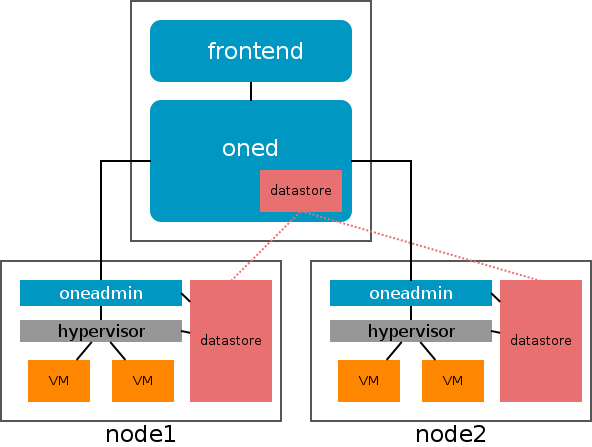
\includegraphics[width=0.8\textwidth]{opennebula-arch.png}
	\end{center}
	\caption{OpenNebula architecture}
	\label{img:opennebula-arch}
\end{figure}

Frontend acts orchestrator and uses additional modules to operate cloud infrastructure. There modules are universal to work with various underlying systems and each module must provide standardized interface for orchestrator. Modules and functions as defined in \cite{opennebula} are:
\begin{description}
	\item[Infrastructure and cloud drivers] enable access to infrastructure and cloud providers
	\item[Virtual machine manager] is used for managing \Ac{VM}s and executing action on them
	\item[Network manager] provide network configuration and management
	\item[Storage manager] supply storage for services and customers
	\item[Image manager] maintain library of \Ac{VM} images
	\item[Information manager] is collecting runtime information about physical infrastructure, \Ac{VM}s and other devices
	\item[Authentication and authorization] is used to authenticate users, store information about them, their permission and quotas
	\item[Accounting and auditing] gather information about resource usage and can be used to generate billing data
	\item[Federation manager] provide mechanism to access remote cloud providers
	\item[Scheduler] manages initial placement of new \Ac{VM}s according to scheduling policy
	\item[Administrative tools] provide interface for users and administrator to perform task on cloud system
	\item[Service manager] can work with group of interconnected \Ac{VM}s as with one service with defined requirements and deployment rules
\end{description}


% control

% datastore

% networkig


-----



% hodit nějakou špínu
